\section{Method}
\label{sec:method}

We introduce \textbf{MASOpt}, an online prompt optimization framework that applies the principle of closed-loop control theory to a fixed multi-agent system.
The key idea is simple.
A prompt update is not treated as a final optimization result.
Instead, it is treated as a temporary intervention whose effect must be measured from the subsequent behavior of the target MAS.
MASOpt combines two complementary stages.
Offline, Cross-Actuation Relative Advantage identifies reusable repair preferences from historical trajectories.
Online, a three-agent meta-MAS repeatedly diagnoses runtime failures, proposes local prompt repairs, and verifies their effects within the same episode.

\begin{figure}[t]
    \centering
    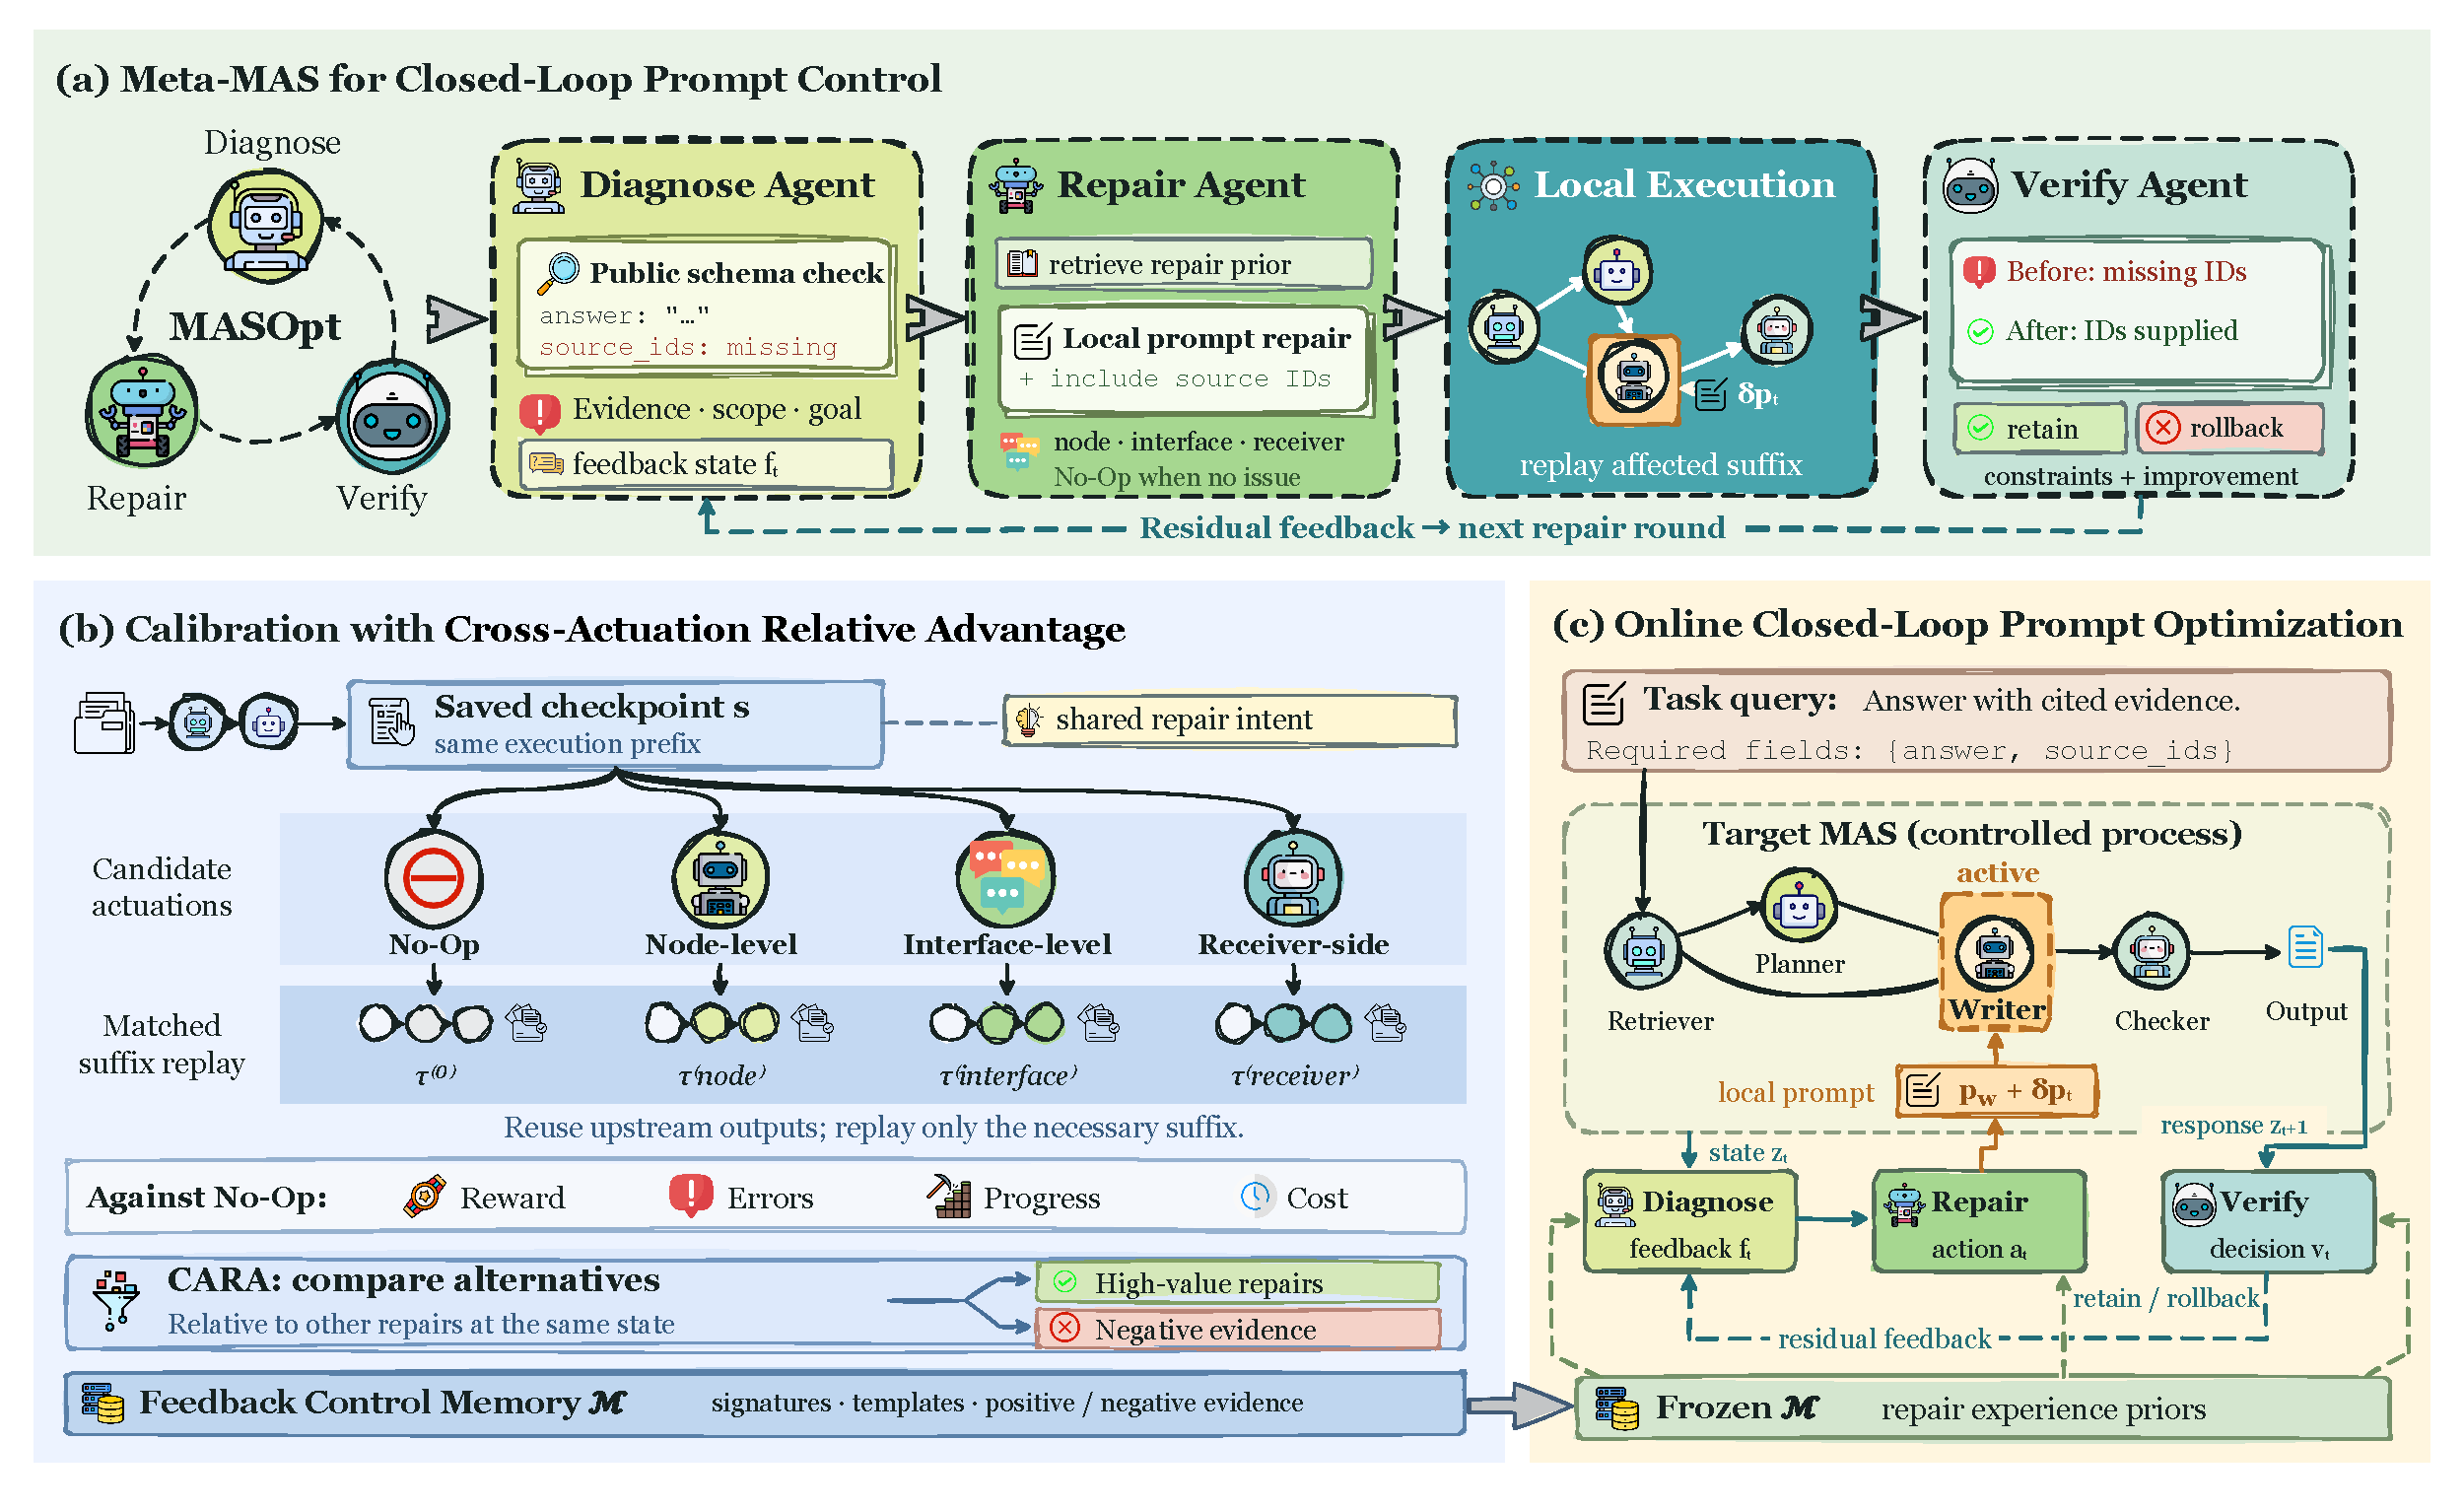
\includegraphics[width=\linewidth]{figures/masopt_method_overview.pdf}
    \caption{Overview of MASOpt. \textbf{(a) A three-agent meta-MAS for closed-loop prompt control} (Section~\ref{sec:meta_agents}): the Diagnose, Repair, and Verify Agents identify failures, propose local prompt repairs, and assess their observable effects. \textbf{(b) Offline calibration with Cross-Actuation Relative Advantage} (Section~\ref{sec:cara}): matched-state probes compare candidate actuations and distill positive and negative evidence into Feedback Control Memory. \textbf{(c) Online closed-loop prompt optimization} (Section~\ref{sec:online}): frozen memory supplies experience priors to the three agents, while prompt interventions at an active MAS node are retained or rolled back based on verification; residual feedback initiates another repair round. The task and agent roles are illustrative.}
    \label{fig:masopt-overview}
\end{figure}


\subsection{Online Prompt Optimization in Multi-Agent Systems}
\label{sec:problem}

\paragraph{Target multi-agent system.}
We consider a fixed multi-agent workflow represented by a directed graph
\begin{equation}
    \mathcal{G}=(\mathcal{V},\mathcal{E}),
\end{equation}
where each node $v_i\in\mathcal{V}$ denotes an agent invocation and each directed edge $(v_i,v_j)\in\mathcal{E}$ represents information passed from an upstream agent to a downstream agent.
The workflow topology and underlying LLMs remain fixed.
Let
\begin{equation}
    \mathbf{P}_0=
    \left(p_1^0,p_2^0,\ldots,p_N^0\right)
\end{equation}
denote the initial prompt configuration associated with the $N$ agents.

For an input task $x$, the target MAS executes according to $\mathcal{G}$ and produces a partial trajectory
\begin{equation}
    \tau_t =
    \left(o_1,o_2,\ldots,o_t\right),
\end{equation}
where $o_t$ may contain an agent response, an inter-agent message, a tool result, an environment observation, or another publicly available execution signal.
We denote the runtime information available to the optimizer by
\begin{equation}
    z_t = \mathcal{O}(x,\tau_t),
\end{equation}
where $\mathcal{O}$ excludes hidden evaluation labels and test-time ground truth.

\paragraph{Prompt intervention.}
Unlike conventional prompt optimization, MASOpt does not assume that $\mathbf{P}_0$ must remain fixed for the complete episode.
At an eligible execution checkpoint, the optimizer may apply a local prompt intervention
$a_t\in\mathcal{A}(z_t)$.
An intervention may modify the instruction of a single agent, an inter-agent interface constraint, a receiver-side rule, or a small local scope of the workflow.
A no-operation action is always available.
If an intervention is accepted, the prompt state becomes
\begin{equation}
    \mathbf{P}_{t+1}
    =
    \mathcal{U}(\mathbf{P}_t,a_t),
    \label{eq:prompt_update}
\end{equation}
where $\mathcal{U}$ applies only the local modification specified by $a_t$.

The goal is to learn an online optimization policy $\pi$ that improves final task utility while avoiding unnecessary interventions,
\begin{equation}
    \max_{\pi}\;
    \mathbb{E}_{x\sim\mathcal{D}}
    \left[
        R(\tau_T)
        -
        \lambda
        \sum_{t=1}^{T} C(a_t)
    \right],
    \qquad
    a_t\sim\pi(\cdot\mid x,z_{\leq t},\mathcal{M}),
    \label{eq:objective}
\end{equation}
where $R$ is the final task metric, $C(a_t)$ measures the cost of an intervention, and $\mathcal{M}$ denotes the repair experience obtained during offline calibration.
Importantly, $R$ is used for development-time learning and final evaluation.
The online policy does not observe hidden task labels during deployment.

\paragraph{Closed-loop view.}
Equation~\ref{eq:objective} differs from standard offline prompt search in one important respect.
The next prompt action depends on the output produced after previous actions.
From the perspective of closed-loop control theory, the target MAS acts as the controlled process, local prompt modifications serve as control inputs, and the observable trajectory provides runtime measurements.
The post-intervention response is fed back into the optimizer before another modification is made.
We use this closed-loop structure as an algorithmic principle and do not assume that LLM-based MAS satisfy linear system dynamics or classical stability conditions.


\subsection{A Three-Agent Meta-MAS for Closed-Loop Prompt Control}
\label{sec:meta_agents}

MASOpt implements the online optimizer with a lightweight meta-MAS containing three specialized agents.
They operate on the target MAS without changing its topology or model parameters.
Each agent has a narrow responsibility so that diagnosis, intervention, and verification remain separated.

\paragraph{\textbf{Diagnose Agent.}}
The Diagnose Agent converts the current execution history into a structured \emph{feedback state}.
Given the task $x$, the observable trajectory $z_{\leq t}$, and retrieved historical experience from $\mathcal{M}$, it produces
\begin{equation}
    f_t =
    \mathcal{D}
    \left(
        x,z_{\leq t};\mathcal{M}
    \right).
    \label{eq:diagnose}
\end{equation}
The feedback state records the detected problem, supporting evidence, its severity, the affected execution scope, and the behavior that should be restored.
Whenever deterministic signals are available, such as syntax errors, failed public tests, missing message fields, or invalid environment actions, they are checked before semantic diagnosis.
The Diagnose Agent therefore identifies \emph{what needs to be corrected} without committing to a particular prompt edit.

\paragraph{\textbf{Repair Agent.}}
The Repair Agent maps the feedback state to a localized prompt intervention.
It conditions on the current prompt state, the diagnosed problem, and historical repair preferences,
\begin{equation}
    a_t =
    \mathcal{R}
    \left(
        f_t,\mathbf{P}_t,z_t;\mathcal{M}
    \right).
    \label{eq:repair}
\end{equation}
Rather than rewriting the entire workflow, the Repair Agent searches over a small action space that targets only the relevant agent or communication interface.
Retrieved experience provides a prior over repair types, but the final text is instantiated using the current task context.
This design keeps interventions small and makes their effects easier to verify.

\paragraph{\textbf{Verify Agent.}}
After a candidate intervention is applied, the affected portion of the target MAS is executed again or allowed to continue until a comparable checkpoint is reached.
The Verify Agent evaluates the new observable state relative to the pre-intervention state, conditioned on applicable experience from the frozen Feedback Control Memory,
\begin{equation}
    v_t =
    \mathcal{V}
    \left(
        f_t,z_t,z_{t+1};\mathcal{M}
    \right),
    \label{eq:verify}
\end{equation}
where $v_t$ contains an acceptance decision and, when necessary, a description of the remaining problem.
Retrieved experience provides a verification prior; the acceptance decision still depends on current observable evidence and hard constraints.
A repair is retained only when the available evidence indicates improvement without violating hard constraints.
A harmful intervention is rolled back.
If the repair resolves only part of the problem, the remaining discrepancy becomes feedback for a subsequent optimization round.

The Verify Agent is therefore not merely a terminal judge.
Its post-intervention assessment determines the next state of the optimizer.
This feedback is what closes the prompt optimization loop.


\subsection{Offline Calibration with Cross-Actuation Relative Advantage}
\label{sec:cara}

Running the online optimizer without prior experience would require repeated exploration at deployment time.
MASOpt therefore uses the training split to estimate which types of local intervention are effective under different execution states.
This stage does not update any LLM parameters.
Instead, it calibrates an external feedback-control memory.

\paragraph{\textbf{Matched-state actuation probing.}}
We first execute the fixed target MAS on calibration tasks and retain a small set of informative checkpoints.
For a checkpoint $s$, MASOpt constructs a repair intent that specifies the behavior to be restored without prescribing where the repair should be applied.
It then generates a candidate set
\begin{equation}
    \mathcal{A}_s =
    \left\{
        a_0,a_1,\ldots,a_K
    \right\},
\end{equation}
where $a_0$ denotes \textsc{No-Op} and the remaining candidates correspond to legal local interventions such as node-level, interface-level, or receiver-side repairs.

All candidates are evaluated from the same saved execution prefix.
Unaffected upstream outputs are reused and only the necessary suffix is replayed.
This matched-state design controls for differences in the preceding trajectory and makes the comparison primarily reflect the effect of the intervention itself.

\paragraph{\textbf{Cross-Actuation Relative Advantage.}}
For an actuation $a$ at state $s$, we define a paired utility
\begin{equation}
\begin{split}
    U(s,a)
    =\;&
    \lambda_R \Delta R(s,a)
    +
    \lambda_E \Delta E(s,a)
    +
    \lambda_P \Delta P(s,a) \\
    &-
    \lambda_C C(s,a),
\end{split}
\label{eq:utility}
\end{equation}
where $\Delta R$ is the task-reward improvement relative to the matched \textsc{No-Op}, $\Delta E$ measures the reduction in observable execution error, $\Delta P$ measures progress toward task completion, and $C$ captures intervention and replay cost.
Ground-truth task reward is used only during offline calibration.

Absolute improvement alone is often difficult to compare across heterogeneous states.
We therefore introduce \textbf{Cross-Actuation Relative Advantage (CARA)}, which evaluates each repair relative to the other candidate interventions generated from the same checkpoint.
Let
\begin{equation}
    \mu_{-a}(s)
    =
    \frac{1}{|\mathcal{A}_s|-1}
    \sum_{\substack{b\in\mathcal{A}_s\\b\neq a}}
    U(s,b)
\end{equation}
and let $\sigma_{-a}(s)$ be the corresponding standard deviation.
CARA is defined as
\begin{equation}
    A_{\mathrm{CARA}}(s,a)
    =
    \frac{
        U(s,a)-\mu_{-a}(s)
    }{
        \sigma_{-a}(s)+\epsilon
    }.
    \label{eq:cara}
\end{equation}
CARA captures whether a repair is unusually effective for the \emph{same execution state}, rather than merely successful in absolute terms.
This distinction is useful in MAS because the component where an error becomes visible is not necessarily the location where intervention is most effective.

\paragraph{\textbf{Feedback Control Memory.}}
High-value repairs are distilled into reusable memory entries.
Each entry records a state or failure signature, the relevant topology context, a repair type, a bounded prompt template, its applicability conditions, and empirical effectiveness statistics.
Repairs that consistently degrade performance are retained as negative evidence rather than discarded.
At deployment time, this memory is frozen and queried only as a prior.
It never stores test answers and is not updated across test tasks.

The resulting memory therefore answers a compact question: given a recognizable execution problem, which form of local prompt intervention has historically been effective, and under what conditions?


\subsection{Online Closed-Loop Prompt Optimization}
\label{sec:online}

At deployment time, MASOpt starts each task from the original prompt configuration $\mathbf{P}_0$ and a frozen Feedback Control Memory $\mathcal{M}$.
No ground-truth answer or hidden evaluation result is available to the online optimizer.

The target MAS first executes normally until an eligible checkpoint is reached.
If the available deterministic and semantic evidence does not indicate a meaningful problem, MASOpt performs no intervention.
Otherwise, the Diagnose Agent constructs a feedback state and retrieves a small number of relevant repair experiences from $\mathcal{M}$.
The Repair Agent uses them to instantiate a minimal intervention for the current execution context.

The intervention is then applied only to the affected part of the workflow.
Whenever the execution environment permits checkpoint replay, unaffected upstream computations are reused.
In other settings, the system continues from the closest valid local state.
This restriction prevents an online repair from degenerating into a complete restart of the MAS.

The Verify Agent evaluates the post-repair behavior using only signals available during execution.
These may include deterministic constraints, public tests, consistency checks, tool responses, environment progress, or structured semantic feedback.
If the new state provides verified improvement, the repaired prompt state is retained.
If it degrades the observable state or violates a hard constraint, MASOpt restores the previous prompt state,
\begin{equation}
    \mathbf{P}_{t+1}
    =
    \begin{cases}
        \mathcal{U}(\mathbf{P}_t,a_t),
        & \text{if } v_t=\textsc{Accept}, \\[3pt]
        \mathbf{P}_t,
        & \text{if } v_t=\textsc{Reject}.
    \end{cases}
    \label{eq:accept}
\end{equation}
When the verification result indicates partial improvement, the remaining problem is incorporated into the next feedback state and the online optimizer may perform another bounded repair round.

This repeated use of post-intervention measurements is the defining distinction between MASOpt and one-shot prompt rewriting.
The online optimizer does not assume that its first repair is correct.
It continuously conditions future prompt decisions on the observed consequences of earlier ones.
All temporary prompt modifications are local to the current episode and are cleared when the task terminates.
As a result, MASOpt realizes online adaptation within a task while preserving a fixed target model, a fixed MAS topology, and a frozen cross-task experience memory.
